\subsection{Basic calculations}
\subsubsection{Addition / subtraction}
$(\mathbf {A}+\mathbf {B})_{i,j}=\mathbf {A}_{i,j}+{\mathbf {B}}_{i,j},\quad 1\leq i\leq m,\quad 1\leq j\leq n$\\
$(\mathbf {A}-\mathbf {B})_{i,j}=\mathbf {A}_{i,j}-{\mathbf {B}}_{i,j},\quad 1\leq i\leq m,\quad 1\leq j\leq n$
\subsubsection{Scalar multiplication}
$(c\mathbf{A})_{i,j}=c\cdot A_{i,j}$
\subsubsection{Matrix multiplication}
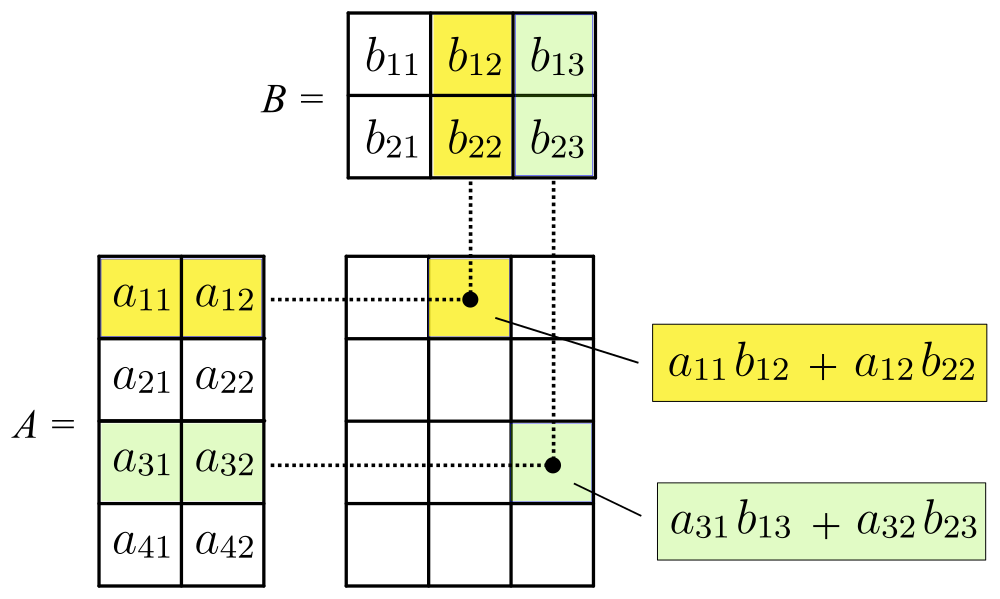
\includegraphics[width=0.35\textwidth]{MatrixMultiplication}

\subsubsection{Transposition}
$(\mathbf{A}^\mathrm{T})_{i,j}=A_{j,i}$


\subsection{Finding determinants}

\subsubsection{$2\times2$ matrices}
$\begin{vmatrix}a&b\\c&d\end{vmatrix}=ad-bc$

\subsubsection{$3\times3$ matrices}

$\begin{vmatrix}a&b&c\\d&e&f\\g&h&i\end{vmatrix}=aei+bfg+cdh-ceg-bdi-afh$
\subsection{Finding inverse matrices}
\subsubsection{$2\times2$ matrices}
$\begin{bmatrix}
	a & b\\c & d
\end{bmatrix}^{-1}=\dfrac{1}{ad-bc}\begin{bmatrix}
	d & -b\\-c & a
\end{bmatrix}$

\subsubsection{$3\times3$ matrices}
$\mathbf {A} ^{-1}={\begin{bmatrix}a&b&c\\d&e&f\\g&h&i\\\end{bmatrix}}^{-1}={\frac {1}{\det(\mathbf {A} )}}{\begin{bmatrix}\,A&\,B&\,C\\\,D&\,E&\,F\\\,G&\,H&\,I\\\end{bmatrix}}^{\mathrm {T} }={\frac {1}{\det(\mathbf {A} )}}{\begin{bmatrix}\,A&\,D&\,G\\\,B&\,E&\,H\\\,C&\,F&\,I\\\end{bmatrix}}$\\
$\begin{alignedat}{6}A&={}&(ei-fh),&\quad &D&={}&-(bi-ch),&\quad &G&={}&(bf-ce),\\B&={}&-(di-fg),&\quad &E&={}&(ai-cg),&\quad &H&={}&-(af-cd),\\C&={}&(dh-eg),&\quad &F&={}&-(ah-bg),&\quad &I&={}&(ae-bd).\\\end{alignedat}$


